\chapter{Trees}
\label{chp:trees}
In this chapter are introduced the fundamentals concepts of tree as abstract data type, and the most used algorithms related to \textbf{trees}.

\section{General Definitions}
A \textbf{tree} is an abstract datatype that simulate a hierarchical structure \cite{wikitrees} (\href{https://en.wikipedia.org/wiki/Tree_(data_structure)}{Trees, Wikipedia}). A tree is a particular kind of a linked list where there are more next elements. The base element of a tree is called \textbf{node} while the first element is called \textbf{root}.

\begin{figure}[H]
\centering
\begin{tikzpicture}[every node/.style={circle,draw}, node distance=15mm, thick]

\draw (0,0) node[draw=none, rectangle, align=left] (r1) {Linked List};
\draw ($(r1) + (-1.5mm, -1)$) node[rectangle, align=left] (r2) {Data: A \\ Next:};
\draw ($(r1) + (2, -1)$) node[rectangle, align=left] (r3) {Data: B \\ Next:};

\draw[->, >=stealth] ($(r2) + (3mm, -3mm)$) -- ($(r3) + (-6.3mm, -3mm)$);

\draw (6,0) node[draw=none, rectangle, align=left] (r4) {Tree};
\draw ($(r4) + (0, -1.2)$) node[align=left] (n1) {Data: C \\ Next:};
\draw ($(n1) + (-2, -2.4)$) node[align=left] (n2) {Data: D \\ Next:};
\draw ($(n1) + (0, -2.4)$) node[align=left] (n3) {Data: E \\ Next:};
\draw ($(n1) + (2, -2.4)$) node[align=left] (n4) {Data: F \\ Next:};

\draw ($(r4) + (-2.2, -0.5)$) node[draw=none, rectangle, align=left] (r5) {\textcolor{ForestGreen}{Root}};
\draw ($(r4) + (2.2, -0.5)$) node[draw=none, rectangle, align=left] (r6) {\textcolor{ForestGreen}{Node}};

\draw[->, >=stealth, ForestGreen] (r5) -- (n1);
\draw[->, >=stealth, ForestGreen] (r6) -- (n1);

\draw[->, >=stealth] (n1) -- (n2);
\draw[->, >=stealth] (n1) -- (n3);
\draw[->, >=stealth] (n1) -- (n4);

\end{tikzpicture}

\caption[Elements of a tree and linked list.]{Elements of a tree and linked list.}
\label{trees_1}
\end{figure}

Trees must be completed connected structures, this means that there are not any nodes which are not connected to anything (Figure \ref{trees_2} case (a)), and there must not be present any cycles (Figure \ref{trees_2} case (c)).

\begin{figure}[H]
\centering
\begin{subfigure}[b]{0.2\linewidth}
\centering
	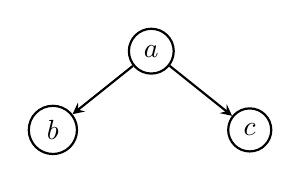
\begin{tikzpicture}[thick, every node/.style={circle,draw}, ->, >=stealth]
    	\node {$a$}
   			child{node {$b$}}
   		 	child{node {$c$}};
	\end{tikzpicture}
	\caption{}
	\label{trees_2_ccc}
\end{subfigure}
\hspace{1em}
\begin{subfigure}[b]{0.2\linewidth}
\centering
	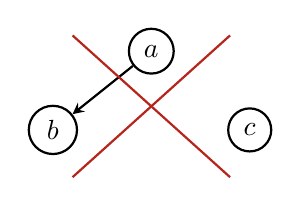
\begin{tikzpicture}[thick, every node/.style={circle,draw}, ->, >=stealth]
		\node {$a$}
   			child{node {$b$}}
   		 	child{node {$c$} edge from parent[draw=none]};
   		
   		\draw[BrickRed, style={-}] (-1,0.2) -- (1,-1.6);
		\draw[BrickRed, style={-}] (1,0.2) -- (-1,-1.6);
	\end{tikzpicture}
	\caption{}
	\label{trees_2_nccc}
\end{subfigure}
\hspace{1em}
\begin{subfigure}[b]{0.2\linewidth}
\centering
	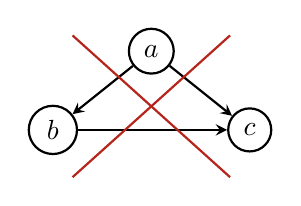
\begin{tikzpicture}[thick, every node/.style={circle,draw}, ->, >=stealth]
		\node {$a$}
   			child{node (ct1) {$b$}}
   		 	child{node (ct2) {$c$}};
   		 \draw[->, >=stealth] (ct1) -- (ct2);  
   		 
   		 \draw[BrickRed, style={-}] (-1,0.2) -- (1,-1.6);
		 \draw[BrickRed, style={-}] (1,0.2) -- (-1,-1.6);
	\end{tikzpicture}
	\caption{}
	\label{trees_2_c}
\end{subfigure}
\caption[Possible structures of a tree.]{Completed connected structure (\ref{trees_2_ccc}), a non completed connected structure (\ref{trees_2_nccc}), and a cycle (\ref{trees_2_c}).}
\label{trees_2}
\end{figure}

Trees are a hierarchical structures divided into layers: the first layer is the one belonging to the root node, the first node of a tree. The next element of the root are called children, which became parents in case they have next node connected as well. The last nodes of a trees are the nodes which do not have any children and they are called \textbf{leaf}. The numbers of connections is called \textbf{height}. A set of connections creates a \textbf{path}. The numbers of edges starting from the root to a node is called \textbf{depth}.
All this definitions are defined in following figure (Figure \ref{trees_3}).

\begin{figure}[H]
\centering
\begin{tikzpicture}[every node/.style={circle,draw}, node distance=15mm, thick]

\node[->, >=stealth] (na){$a$}
   child{node (nb) {$b$} edge from parent[->, >=stealth]
             child {node (nd) {$d$} edge from parent[->, >=stealth]}
             child {node (ne) {$e$} edge from parent[->, >=stealth]}
        }
   child{node (nc) {$c$} edge from parent[->, >=stealth]
			child[missing]
			child{node (nf) {$f$}} edge from parent[->, >=stealth]
		};
\draw ($(na) + (0, 1)$) node[draw=none, rectangle, align=left] (r5) {Root};
\draw ($(na) + (-1.5, 0)$) node[draw=none, rectangle, align=left] (r6) {Node};
\draw ($(na) + (1.6, -0.4)$) node[draw=none, rectangle, align=left] (r7) {Edge};
\draw ($(nb) + (-1.6, 0.4)$) node[draw=none, rectangle, align=left] (r8) {Parent};
\draw ($(nd) + (-1.8, 0.4)$) node[draw=none, rectangle, align=left] (r9) {\textcolor{ForestGreen}{Subtree}};
\draw ($(nb) + (0,-2.6)$) node[draw=none, rectangle, align=left] (r10) {Children};
\draw ($(nf) + (1,1)$) node[draw=none, rectangle, align=left] (r11) {Leaf node};
\draw ($(nc) + (4,0)$) node[draw=none, rectangle, align=left] (r12) {Height \\ of the \\ tree};

\draw[->, >=stealth] (r5) -- (na);
\draw[->, >=stealth] (r6) -- ($(na) + (-1mm, 0)$);
\draw[->, >=stealth] (r7) -- ($(na) + (0.4, -0.6)$);
\draw[->, >=stealth] (r8) -- (nb);
\draw[->, >=stealth, ForestGreen] (r9) -- ($(nd) + (-0.9,-0.3)$);
\draw[->, >=stealth] (nd) -- (r10);
\draw[->, >=stealth] (ne) -- (r10);
\draw[->, >=stealth] (nf) -- (r11);
\draw[<->, >=stealth] ($(nf) + (2.5,3.2)$) -- ($(nf) + (2.5,-0.3)$);

\draw[ForestGreen, rounded corners, dashed, line width=1pt]
    ($(nb) + (0,0.8)$) --
    ($(nd) + (-1,-0.5)$) --
    ($(ne) + (1,-0.5)$) --
    ($(nb) + (0,0.8)$);

\end{tikzpicture}
\caption[A tree and its fundamentals elements.]{A tree and its fundamentals elements.}
\label{trees_3}
\end{figure}

\section{Tree Traversal}
Which way is the most efficient for visiting all the nodes of a tree? Is it more efficient looking layer by layer or looking at subtrees? There are two different approach to traverse a tree: the \textbf{depth-first search} (\textbf{DFS}) and the \textbf{breadth-first search} (\textbf{BFS}). In the first one the priority is to look at the children of a node, instead in the second one the priority is to look at the node of the same layer \ref{trees_4}.

\begin{figure}[H]
\centering
\begin{subfigure}[b]{0.4\linewidth}
\centering
\begin{tikzpicture}[every node/.style={circle,draw}, node distance=15mm, thick]

\node[->, >=stealth] (na){$a$}
   child{node (nb) {$b$} edge from parent[->, >=stealth]
             child {node (nd) {$d$} edge from parent[->, >=stealth]}
             child {node (ne) {$e$} edge from parent[->, >=stealth]}
        }
   child{node (nc) {$c$} edge from parent[->, >=stealth]
			child[missing]
			child{node (nf) {$f$}} edge from parent[->, >=stealth]
		};

\draw[ForestGreen, line width=1pt]
    ($(nb) + (0,0.8)$) --
    ($(nd) + (-1,-0.5)$) --
    ($(ne) + (1,-0.5)$) --
    ($(nb) + (0,0.8)$);

\end{tikzpicture}
\caption{}
\label{dfs}
\end{subfigure}
\hspace{1em}
\begin{subfigure}[b]{0.4\linewidth}
\centering
\begin{tikzpicture}[every node/.style={circle,draw}, node distance=15mm, thick]

\node[->, >=stealth] (na){$a$}
   child{node (nb) {$b$} edge from parent[->, >=stealth]
             child {node (nd) {$d$} edge from parent[->, >=stealth]}
             child {node (ne) {$e$} edge from parent[->, >=stealth]}
        }
   child{node (nc) {$c$} edge from parent[->, >=stealth]
			child[missing]
			child{node (nf) {$f$}} edge from parent[->, >=stealth]
		};

\draw[ForestGreen, line width=1pt]
    ($(nb) + (-0.5,0.6)$) --
    ($(nb) + (-0.5,-0.6)$) --
    ($(nc) + (0.5,-0.6)$) --
    ($(nc) + (0.5,0.6)$) --
    ($(nb) + (-0.5,0.6)$);

\end{tikzpicture}
\caption{}
\label{bfs}
\end{subfigure}
\caption[The depth-first search (\ref{dfs}) and the breadth-first search (\ref{bfs}).]{The depth-first search (\ref{dfs}) and the breadth-first search (\ref{bfs})}
\label{trees_4}
\end{figure}

AGGIUNGERE LA COMPLESSITÀ COMPUTAZIONALE DEI DUE APPROCCI.

\subsection{Depth-first search}
In the depth-first search there are several different ways to perform a search on a tree. AGGIUNGERE LO SPANNING TREE E IL METODO DI RICERCA: VISIT, LEFT, RIGHT...
\paragraph{Pre-order search}
\label{preorder}
In the \textbf{pre-order search} the first node to be checked as visited is the root. The following node is the left child by convention. Once checked the left child the process is repeated until the first node without any children is reached. At that point the same process is applied to the right side: all the nodes on the right are checked until all the nodes are checked as visited \ref{trees_5}.

\begin{figure}[H]
\centering
\begin{tikzpicture}[every node/.style={circle,draw}, node distance=15mm, thick]

\node (na){$a$}
   child{node (nb) {$b$}
             child {node (nd) {$d$}}
             child {node (ne) {$e$}}
        }
   child{node (nc) {$c$}
			child[missing]
			child{node (nf) {$f$}}
		};
\draw ($(na) + (-2, 0.4)$) node[rectangle] {Pre-order};
\draw node[draw=none, rectangle, below=1mm of nd] {a, b, d, e, c, f};
  
  %\fill circle (3pt) node ($(na) + (-0.4,0.2)$) {Here!};
  \fill[color=black] ($(na) + (-0.42,0.2)$) circle (0.1);
  \fill[color=black] ($(nb) + (-0.42,0.2)$) circle (0.1);
  \fill[color=black] ($(nd) + (-0.48,0.0)$) circle (0.1);
  \fill[color=black] ($(ne) + (-0.45,0.0)$) circle (0.1);
  \fill[color=black] ($(nc) + (-0.5,0.15)$) circle (0.1);
  \fill[color=black] ($(nf) + (-0.48,0.0)$) circle (0.1);
  
  \draw[->, >=stealth, BrickRed, rounded corners, dashed, line width=0.7pt]
    ($(na) + (-0.4,0.2)$) --
    ($(nb) + (-0.4,0.2)$) --
    %($(nb) + (-0.44,0.0)$) --
    ($(nd) + (-0.50,0.0)$) --
    ($(nd) + (-0.35,-0.35)$) --
    ($(nd) + (0.0,-0.45)$) --
    ($(nd) + (0.35,-0.35)$) --
    ($(nd) + (0.42,0.0)$) --
    ($(nb) + (0.0,-0.4)$) --
    ($(ne) + (-0.45,0.0)$) --
    ($(ne) + (-0.35,-0.35)$) --
    ($(ne) + (0.0,-0.45)$) --
    ($(ne) + (0.35,-0.35)$) --
    ($(ne) + (0.45,0.0)$) --
    ($(nb) + (0.4,0.0)$) --
    ($(na) + (0.0,-0.4)$) --
    ($(nc) + (-0.5,0.15)$) --
    ($(nf) + (-0.45,0.0)$) --
    ($(nf) + (-0.35,-0.35)$);
    %($(nf) + (0.0,-0.45)$) --
    %($(nf) + (0.35,-0.35)$);
    %($(nf) + (0.48,0.0)$) --
    %($(nc) + (0.42,-0.4)$);
    %($(nc) + (0.36,0.4)$) --
    %($(na) + (0.4,0.2)$);
\end{tikzpicture}

\caption[Pre-order search.]{Pre-order search.}
\label{trees_5}
\end{figure}

\paragraph{In-order search}
\label{inorder}
In the \textbf{in-order search} the first node to be checked is the first node without children on the left side (or right side). Once checked off this node the next one to be checked off is its parent, and the process is repeated again on the right side of the nodes, until all the nodes are checked off.

\begin{figure}[H]
\centering
\begin{tikzpicture}[every node/.style={circle,draw}, node distance=15mm, thick]

\node (na){$a$}
   child{node (nb) {$b$}
             child {node (nd) {$d$}}
             child {node (ne) {$e$}}
        }
   child{node (nc) {$c$}
			child[missing]
			child{node (nf) {$f$}}
		};
\draw ($(na) + (-2, 0.4)$) node[rectangle] {In-order};
\draw node[draw=none, rectangle, below=1mm of nd] {d, b, e, a, c, f};
  
  %\fill circle (3pt) node ($(na) + (-0.4,0.2)$) {Here!};
  \fill[color=black] ($(nd) + (-0.48,0.0)$) circle (0.1);
  \fill[color=black] ($(nb) + (0.0,-0.5)$) circle (0.1);
  \fill[color=black] ($(ne) + (-0.45,0.0)$) circle (0.1);
  \fill[color=black] ($(na) + (0.0,-0.5)$) circle (0.1);
  \fill[color=black] ($(nf) + (-0.48,0.0)$) circle (0.1);
  \fill[color=black] ($(nc) + (-0.5,0.15)$) circle (0.1);
  
  \draw[->, >=stealth, BrickRed, rounded corners, dashed, line width=0.7pt]
    ($(na) + (-0.4,0.2)$) --
    ($(nb) + (-0.4,0.2)$) --
    %($(nb) + (-0.44,0.0)$) --
    ($(nd) + (-0.50,0.0)$) --
    ($(nd) + (-0.35,-0.35)$) --
    ($(nd) + (0.0,-0.45)$) --
    ($(nd) + (0.35,-0.35)$) --
    ($(nd) + (0.42,0.0)$) --
    ($(nb) + (0.0,-0.4)$) --
    ($(ne) + (-0.45,0.0)$) --
    ($(ne) + (-0.35,-0.35)$) --
    ($(ne) + (0.0,-0.45)$) --
    ($(ne) + (0.35,-0.35)$) --
    ($(ne) + (0.45,0.0)$) --
    ($(nb) + (0.4,0.0)$) --
    ($(na) + (0.0,-0.4)$) --
    ($(nc) + (-0.5,0.15)$) --
    ($(nf) + (-0.45,0.0)$) --
    ($(nf) + (-0.35,-0.35)$);
    %($(nf) + (0.0,-0.45)$);
    %($(nf) + (0.35,-0.35)$);
    %($(nf) + (0.48,0.0)$);
    %($(nc) + (0.64,-0.4)$) --
    %($(nc) + (0.30,0.4)$);
    %($(na) + (0.4,0.2)$);
\end{tikzpicture}
\caption[In-order search.]{In-order search.}
\label{trees_6}
\end{figure}

\paragraph{Post-order search}
\label{postorder}
In the \textbf{post-order search} the first node to be checked off is the first node without children on the left side (or right side). Once checked off this node the next one to be checked off is the one which does not have any children. Once all the nodes of the current left subtree without any children are checked off, the parents can be checked off, and the whole process is repeated until all the nodes are checked off.

\begin{figure}[H]
\centering
\begin{tikzpicture}[every node/.style={circle,draw}, node distance=15mm, thick]

\node (na){$a$}
   child{node (nb) {$b$}
             child {node (nd) {$d$}}
             child {node (ne) {$e$}}
        }
   child{node (nc) {$c$}
			child[missing]
			child{node (nf) {$f$}}
		};
\draw ($(na) + (-2, 0.4)$) node[rectangle] {Post-order};
\draw node[draw=none, rectangle, below=1mm of nd] {d, e, b, f, c, a};
  
  %\fill circle (3pt) node ($(na) + (-0.4,0.2)$) {Here!};
  \fill[color=black] ($(nd) + (-0.48,0.0)$) circle (0.1);
  \fill[color=black] ($(ne) + (-0.45,0.0)$) circle (0.1);
  \fill[color=black] ($(nb) + (0.45,0.0)$) circle (0.1);
  \fill[color=black] ($(nf) + (-0.48,0.0)$) circle (0.1);
  \fill[color=black] ($(nc) + (0.44,0.0)$) circle (0.1);
  \fill[color=black] ($(na) + (0.5,0.0)$) circle (0.1);
  
  \draw[->, >=stealth, BrickRed, rounded corners, dashed, line width=0.7pt]
    ($(na) + (-0.4,0.2)$) --
    ($(nb) + (-0.4,0.2)$) --
    %($(nb) + (-0.44,0.0)$) --
    ($(nd) + (-0.50,0.0)$) --
    ($(nd) + (-0.35,-0.35)$) --
    ($(nd) + (0.0,-0.45)$) --
    ($(nd) + (0.35,-0.35)$) --
    ($(nd) + (0.42,0.0)$) --
    ($(nb) + (0.0,-0.4)$) --
    ($(ne) + (-0.45,0.0)$) --
    ($(ne) + (-0.35,-0.35)$) --
    ($(ne) + (0.0,-0.45)$) --
    ($(ne) + (0.35,-0.35)$) --
    ($(ne) + (0.45,0.0)$) --
    ($(nb) + (0.4,0.0)$) --
    ($(na) + (0.0,-0.4)$) --
    ($(nc) + (-0.5,0.15)$) --
    ($(nf) + (-0.45,0.0)$) --
    ($(nf) + (-0.35,-0.35)$) --
    ($(nf) + (0.0,-0.45)$) --
    ($(nf) + (0.35,-0.35)$) --
    ($(nf) + (0.48,0.0)$) --
    ($(nc) + (0.64,-0.4)$) --
    ($(nc) + (0.30,0.4)$) --
    ($(na) + (0.3,0.4)$);
\end{tikzpicture}
\caption[Post-order search.]{Post-order search.}
\label{trees_7}
\end{figure}

\section{Binary Trees}
\textbf{Binary trees} are trees in which the parent has at most two children (0, 1, 2 are the only number of admitted children). On binary trees some operations like searching, deleting, and inserting can be easily and efficiently done. 
\subsection{Search}
To search an element in the tree one of the previous methods can be used. Because in a general tree there is no ordering this means that potentially all the elements of the tree can be visited, then the complexity results in \(O(n)\).

\begin{figure}[H]
\centering
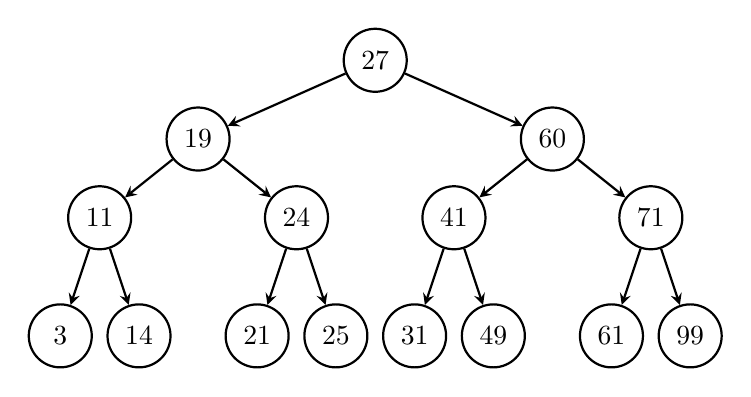
\begin{tikzpicture}[every node/.style={circle,draw,minimum size=8mm}, node distance=15mm, thick, ->, >=stealth]

\tikzstyle{level 1}=[level distance=10mm, sibling distance=4.5cm]
\tikzstyle{level 2}=[level distance=10mm, sibling distance=2.5cm]
\tikzstyle{level 3}=[level distance=15mm, sibling distance=1cm]
\tikzstyle{level 4}=[level distance=15mm, sibling distance=1cm]


\node {$27$}
   child{node {$19$}
             child {node {$11$}
					child{node {$3$}}
					child{node {$14$}}             	
             	}
             child {node {$24$}
                	child{node {$21$}}
					child{node {$25$}}
                }
        }
   child{node {$60$}
			child {node {$41$}
				   child{node {$31$}}
				   child{node {$49$}}             	
             	}
            child {node {$71$}
                   child{node {$61$}}
				   child{node {$99$}}
                }
		};
  
\end{tikzpicture}
\caption[Example of tree search and traversal.]{Example of tree search and traversal.}
\label{trees_12}
\end{figure}

\begin{table}[H]
	\centering
	\begin{tabular}{l  l}
 		 DFS & \\
		\hline
		Pre-order traversal & [27, 19, 11, 3, 14, 24, 21, 25, 60, 41, 31, 49, 71, 61, 99] \\
		In-order traversal & [3, 11, 14, 19, 21, 24, 25, 27, 31, 41, 49, 60, 61, 71, 99] \\
		Post-order & [3, 14, 11, 21, 25, 24, 19, 31, 49, 41, 61, 99, 71, 60, 27] \\
		\hline
		BRF & [27, 19, 60, 11, 24, 41, 71, 3, 14, 21, 25, 31, 49, 61, 99]
	\end{tabular}
\caption[Traversal paths for the tree in Figure \ref{trees_12}.]{Traversal paths for the tree in Figure \ref{trees_12}.}
\end{table}

\subsection{Delete}
Before the delete process there is always a search one for finding the element to be deleted. If the element to be deleted is a leaf, deleting it is not a problem because there are not any children to be moved. Instead if the node to be removed has some children there are several opportunities to reorganize the nodes, because the condition for a binary tree must remain valid (a node can have at most two nodes). So there are several strategies. Let us consider the following tree \ref{trees_9}. 
\begin{itemize}
\item If the node to be removed has only one child it can be replaced by the child node (case 1 Figure \ref{trees_9}).
\item If the node to be removed has two children it can be replaced with the child node which has no children node (case 2 Figure \ref{trees_9}).
\item If the node to be removed has two children which have again children as well, in this case there are several options which can be done. For example on child node can be moved to the position of the one to be removed (case 3 Figure \ref{trees_9}).
\end{itemize} 

\begin{figure}[H]
\centering
\begin{tikzpicture}[every node/.style={circle,draw, minimum size=8mm}, node distance=15mm, thick, ->, >=stealth]

\tikzstyle{level 1}=[level distance=10mm, sibling distance=4.5cm]
\tikzstyle{level 2}=[level distance=10mm, sibling distance=2.5cm]
\tikzstyle{level 3}=[level distance=15mm, sibling distance=1cm]
\tikzstyle{level 4}=[level distance=15mm, sibling distance=1cm]

\node (na){$a$}
   child{node (nb) {$b$}
             child {node (nd) {$d$}
				child{node[BrickRed] (ng) {$g$} edge from parent[BrickRed]}
				child{node[BrickRed] (nh) {$h$} edge from parent[BrickRed]}             
             }
             child {node (ne) {$e$}
             	child{node[BrickRed] (ni) {$i$} edge from parent[BrickRed]}
				child{node[BrickRed] (nj) {$j$} edge from parent[BrickRed]}
             }
        }
   child{node (nc) {$c$}
			child[missing]
			child{node (nf) {$f$}}
		};

\draw[BrickRed, style={-}] ($(nb) + (0.5,0.5)$) -- ($(nb) + (-0.5,-0.5)$);
\draw[BrickRed, style={-}] ($(nb) + (-0.5,0.5)$) -- ($(nb) + (0.5,-0.5)$);

\draw[BrickRed, style={-}] ($(nc) + (0.5,0.5)$) -- ($(nc) + (-0.5,-0.5)$);
\draw[BrickRed, style={-}] ($(nc) + (-0.5,0.5)$) -- ($(nc) + (0.5,-0.5)$);

\path[->, >=stealth, BrickRed] (nf.north east) edge [bend right=60] node[draw=none, xshift=24pt] {Case 1} (nc.east);
\path[->, >=stealth, BrickRed] (ne.north east) edge [bend right=60] node[draw=none, xshift=24pt] {Case 2} (nb.east);
\path[->, >=stealth, BrickRed] (ng.north west) edge [bend left=100] node[draw=none, xshift=-22pt] {Case 3} (nb.west);

\end{tikzpicture}
\caption[Delete an element of a tree.]{Delete an element of a tree.}
\label{trees_9}
\end{figure}

AGGIUNGERE IL LIBRO DI ALGORITMI CITANDO CHE SIA UNA LETTURA APPROFONDITA PER MAGGIORI DETTAGLI.
\subsection{Insert}
Insert a new element to a binary tree is not a hard operation, because it is enough to find a node which can take a new children node. In the worst case to find the proper node in which a child can be add the farthest leaf must be reached (case 1 \ref{trees_10}).

\begin{figure}[H]
\centering
\begin{tikzpicture}[every node/.style={circle,draw, minimum size=8mm}, node distance=15mm, thick]

\tikzstyle{level 1}=[level distance=10mm, sibling distance=4.5cm]
\tikzstyle{level 2}=[level distance=10mm, sibling distance=2.5cm]
\tikzstyle{level 3}=[level distance=15mm, sibling distance=1cm]
\tikzstyle{level 4}=[level distance=15mm, sibling distance=1cm]

\node (na){$a$}
   child{node (nb) {$b$} edge from parent[->, >=stealth]
             child {node (nd) {$d$} edge from parent[->, >=stealth]
				child {node (nh) {$h$} edge from parent[->, >=stealth]}
				child[missing]             
             }
             child {node (ne) {$e$} edge from parent[->, >=stealth]}
        }
   child{node (nc) {$c$} edge from parent[->, >=stealth]
			child{node[BrickRed] (ng) {$g$} edge from parent[BrickRed, ->, >=stealth]}
			child{node (nf) {$f$} edge from parent[->, >=stealth]}
		};

\draw[BrickRed, style={-}, dashed] 
	($(na) + (0.5,0.5)$) -- 
	($(na) + (-0.5,0.5)$) --
	($(na) + (-0.5,-0.5)$) --
	($(na) + (0.5,-0.5)$) --
	($(na) + (0.5,0.5)$);

\draw[BrickRed, style={-}, dashed] 
	($(nb) + (0.5,0.5)$) -- 
	($(nb) + (-0.5,0.5)$) --
	($(nb) + (-0.5,-0.5)$) --
	($(nb) + (0.5,-0.5)$) --
	($(nb) + (0.5,0.5)$);

\draw[BrickRed, style={-}, dashed] 
	($(nd) + (0.5,0.5)$) -- 
	($(nd) + (-0.5,0.5)$) --
	($(nd) + (-0.5,-0.5)$) --
	($(nd) + (0.5,-0.5)$) --
	($(nd) + (0.5,0.5)$);

\draw[BrickRed, style={-}, dashed] 
	($(nh) + (0.5,0.5)$) -- 
	($(nh) + (-0.5,0.5)$) --
	($(nh) + (-0.5,-0.5)$) --
	($(nh) + (0.5,-0.5)$) --
	($(nh) + (0.5,0.5)$);
	
\draw ($(nh) + (1,0)$) node[draw=none, BrickRed, minimum size=2mm, style={-}] {$1$};

\draw[BrickRed, style={-}, dashed] 
	($(nc) + (0.5,0.5)$) -- 
	($(nc) + (-0.5,0.5)$) --
	($(nc) + (-0.5,-0.5)$) --
	($(nc) + (0.5,-0.5)$) --
	($(nc) + (0.5,0.5)$);


\end{tikzpicture}
\caption[Add an element of a tree.]{Add an element of a tree.}
\label{trees_10}
\end{figure}

AGGIUNGERE IL LIBRO DI ALGORITMI CITANDO CHE SIA UNA LETTURA APPROFONDITA PER MAGGIORI DETTAGLI.
\subsection{Perfect binary tree}
A perfect binary tree is a binary tree in which all the nodes have two children except the leaf which do not have any children. In this case the following results are valid

\begin{figure}[H]
\centering
\begin{subfigure}[b]{0.4\linewidth}
\centering
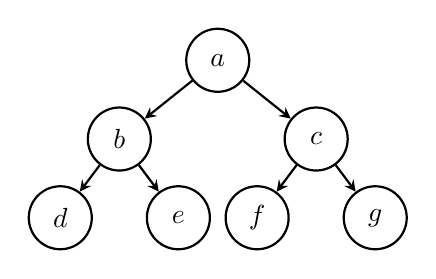
\begin{tikzpicture}[every node/.style={circle,draw, minimum size=8mm}, node distance=15mm, thick]

\tikzstyle{level 1}=[level distance=10mm, sibling distance=2.5cm]
\tikzstyle{level 2}=[level distance=10mm, sibling distance=1.5cm]
\tikzstyle{level 3}=[level distance=15mm, sibling distance=1cm]
\tikzstyle{level 4}=[level distance=15mm, sibling distance=1cm]

\node (na){$a$}
   child{node (nb) {$b$} edge from parent[->, >=stealth]
             child {node (nd) {$d$} edge from parent[->, >=stealth]}
             child {node (ne) {$e$} edge from parent[->, >=stealth]}
        }
   child{node (nc) {$c$} edge from parent[->, >=stealth]
			child{node (nf) {$f$} edge from parent[->, >=stealth]}
			child{node (ng) {$g$} edge from parent[->, >=stealth]}
		};
\end{tikzpicture}
\end{subfigure}
\hspace{1em}
\begin{subfigure}[b]{0.4\linewidth}
\centering
\begin{tabular}[b]{c c c}
 Level & \# of nodes & Total nodes  \\
\hline
1 & $2^{0}$ & 1 \\
2 & $2^{1}$ & 3 \\
3 & $2^{2}$ & 7
\end{tabular}
\end{subfigure}
\caption[Perfect binary tree.]{Perfect binary tree.}
\label{trees_11}
\end{figure}

When a new row is added, the number of nodes double. Given a level \(n\) the total number of nodes is \(2n + 1\).

\subsection{Binary Tree Implementation}
The following code is the recursive Python implementation of the pre-order search and traversal (Figure \ref{trees_5}). The recursive and iterative implementations of the other ways of search and traverse a tree are in appendix \ref{binappendix}.

\begin{lstlisting}[firstnumber=1, caption={Class definition for a node and a tree.}]
class Node():

	def __init__(self, value):
		self.value = value
		self.left = None
		self.right = None

class BinaryTree():

	def __init__(self, root):
		self.root = Node(root)
\end{lstlisting}

\begin{lstlisting}[firstnumber=1, caption={Recursive pre-order traversal and search implementation.}]
class Node():
	...

class BinaryTree():
	...

	def print_tree(self):
		return self.preorder_print(tree.root, "")[:-1]

	def preorder_search_recursive(self, start, find_val):
		if start:
			if start.value == find_val:
				return True
			self.preorder_search_recursive(start.left, find_val)
			self.preorder_search_recursive(start.right, find_val)	
	
	def preorder_print(self, start, traversal):
		if start:
			traversal += (str(start.value) + "-")
			traversal = self.preorder_print(start.left, traversal)
			traversal = self.preorder_print(start.right,traversal)
		return traversal
\end{lstlisting}

\section{Binary Search Trees (BST)}
Performing operations such as search, addition, or removal of an element it is a very efficient process if the binary tree is ordered. A binary tree is ordered if for all nodes the left child has a minor value, and the right child has a greater value than the considered node \cite{wikibinsearchtree}(\href{https://en.wikipedia.org/wiki/Binary_search_tree}{Binary search tree, Wikipedia}).

\begin{figure}[H]
\centering
\begin{tikzpicture}[every node/.style={circle,draw, minimum size=8mm}, node distance=15mm, thick]

\tikzstyle{level 1}=[level distance=10mm, sibling distance=2.5cm]
\tikzstyle{level 2}=[level distance=10mm, sibling distance=1.5cm]
\tikzstyle{level 3}=[level distance=15mm, sibling distance=1cm]
\tikzstyle{level 4}=[level distance=15mm, sibling distance=1cm]

\node[BrickRed] (n5){$5$}
   child{node (n3) {$3$} edge from parent[->, >=stealth]
             child {node (n1) {$1$} edge from parent[->, >=stealth]}
			 child[missing]
        }
   child{node[BrickRed] (n8) {$8$} edge from parent[->, >=stealth]
			child{node[BrickRed] (n7) {$7$} edge from parent[->, >=stealth]}
			child{node (n10) {$10$} edge from parent[->, >=stealth]}
		};

\draw ($(n5) + (0.6, 0.6)$) node[draw=none, rectangle] {\textcolor{BrickRed}{5<7}};
\draw ($(n8) + (0.6, 0.6)$) node[draw=none, rectangle] {\textcolor{BrickRed}{8>7}};
\draw ($(n7) + (-0.5, 0.6)$) node[draw=none, rectangle] {\textcolor{BrickRed}{7=7}};

\end{tikzpicture}
\caption[Search on an ordered binary tree.]{Search on an ordered binary tree.}
\label{trees_13}
\end{figure}

For example in Figure \ref{trees_13} is an ordered tree. Let us consider we would like to find the node which value is 7. Because the tree is ordered for efficiently finding 7 is enough to compare 7 with the value of the node and choose every time if to search on the right or on the left. In this way for finding a value is not mandatory to look at all the nodes, and the complexity for this operation is \(log(n)\).

Let us consider instead we would like to add a new node of value 4 to the tree of Figure \ref{trees_13}. Because the tree is ordered, there is only one place in which the node can be added. In the case of the tree in Figure \ref{trees_13} the node can be easily added because there is an empty space that can correctly take it (Figure \ref{trees_14}). In this case the complexity for this operation is again \(log(n)\).

\begin{figure}[H]
\centering
\begin{tikzpicture}[every node/.style={circle,draw, minimum size=8mm}, node distance=15mm, thick]

\tikzstyle{level 1}=[level distance=10mm, sibling distance=2.5cm]
\tikzstyle{level 2}=[level distance=10mm, sibling distance=1.5cm]
\tikzstyle{level 3}=[level distance=15mm, sibling distance=1cm]
\tikzstyle{level 4}=[level distance=15mm, sibling distance=1cm]

\node[BrickRed] (n5){$5$}
   child{node[BrickRed] (n3) {$3$} edge from parent[->, >=stealth]
             child {node (n1) {$1$} edge from parent[->, >=stealth]}
			 child {node[BrickRed] (n4) {$4$} edge from parent[->, >=stealth]}
        }
   child{node(n8) {$8$} edge from parent[->, >=stealth]
			child{node (n7) {$7$} edge from parent[->, >=stealth]}
			child{node (n10) {$10$} edge from parent[->, >=stealth]}
		};

\draw ($(n5) + (-0.6, 0.6)$) node[draw=none, rectangle] {\textcolor{BrickRed}{5<7}};
\draw ($(n3) + (-0.6, 0.6)$) node[draw=none, rectangle] {\textcolor{BrickRed}{8>7}};

\end{tikzpicture}
\caption[Addition on an ordered binary tree.]{Addition on an ordered binary tree.}
\label{trees_14}
\end{figure}

In case the position of the node is already occupied, adding the node could be a very difficult task. For a more complete and formal description of this topic refer to \cite{goodrich2013data} in the chapter about trees.

When all the possible nodes are present in each level the tree is said \textbf{balanced}. In Figure \ref{trees_14} there is an example of a balanced tree.
When instead a tree has all its children nodes which have always a bigger value, all the tree is on the right, and it is said to be \textbf{unbalanced}. In this case the search of an element has a \(O(n)\) complexity in the worst case.

\begin{figure}[H]
\centering
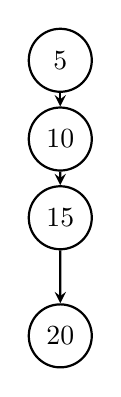
\begin{tikzpicture}[every node/.style={circle,draw, minimum size=8mm}, node distance=15mm, thick]

\node(n5){$5$}
   child{node(n10) {$10$} edge from parent[->, >=stealth]
         child {node (n15) {$15$} edge from parent[->, >=stealth]
		 child{node (n20) {$20$} edge from parent[->, >=stealth]}             
             }
        };

\end{tikzpicture}
\caption[An unbalanced binary tree.]{An unbalanced binary tree.}
\label{trees_15}
\end{figure}

\subsection{Binary Search Tree Implementation}
The following code is the python implementation of the search and addition operations performed on a ordered binary tree.

\begin{lstlisting}[firstnumber=1, caption={implementation of insert and search operation for a binary search tree.}]
class BST():

	def __init__(self, root):
		self.root = Node(root)

	def insert(self, new_val):
		self.insert_helper(self.root, new_val)
	
	def insert_helper(self, current, new_val):
		if current.value < new_val:
			if current.right:
				self.insert_helper(current.right, new_val)
			else:
				self.current.right = Node(new_val)
		else:
			if current.left:
				self.insert_helper(current.left, new_val)
			else:
				current.left = Node(new_val)
	
	def search(self, find_val):
		return self.search_helper(self.root, find_val)
	
	def search_helper(self, current, find_val):
		if current:
			if current.value == find_val:
				return True
			elif current.value < find_val:
				return self.search_helper(current.right, find_val)
			else:
				return self.search_helper(current.left, find_val)
		return False
\end{lstlisting}

\section{Heaps}
\textbf{Heaps} are particular tree-based data structure in which the elements are ordered in increasing or decreasing order \cite{wikiheap} (\href{https://en.wikipedia.org/wiki/Heap_(data_structure)}{Heap, Wikipedia}). Heaps are a very efficient implementation of the abstract data type (Chapter \ref{chp:datastrucutres}) priority queue (Section \ref{queue}). The value with the highest (or lowest) priority is always stored at the root. Heaps are very useful when an element with a high (or low) priority must be repeatedly removed from the heap. Moreover, heaps are not sorted structure, but are regarded as partially ordered.    

We say the \textit{max heap} (Figure \ref{max_heap}) if for every node its children have the values less or equal than the one of the parent (the root has always the highest value). We say instead \textit{min heap} (Figure \ref{min_heap}) if for every node its children have the values higher or equal than the on of the parent (the root has the lowest value).

\begin{figure}[H]
\centering
\begin{subfigure}[b]{0.4\linewidth}
\centering
	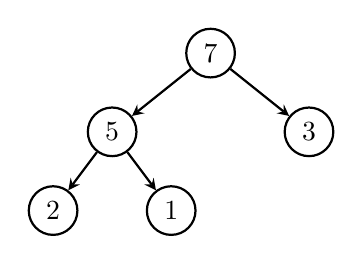
\begin{tikzpicture}[thick, every node/.style={circle,draw}, ->, >=stealth]
		\node {$7$}
   			child{node {$5$}
				child{node {$2$}}
				child{node {$1$}}  			
   			}
   		 	child{node {$3$}};
	\end{tikzpicture}
	\caption{}
	\label{max_heap}
\end{subfigure}
\hspace{1em}
\begin{subfigure}[b]{0.4\linewidth}
\centering
	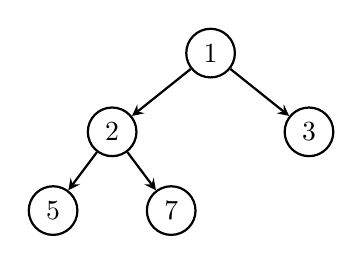
\begin{tikzpicture}[thick, every node/.style={circle,draw}, ->, >=stealth]
		\node {$1$}
   			child{node {$2$}
				child{node {$5$}} 
				child{node {$7$}}   			
   			}
   		 	child{node {$3$}};
	\end{tikzpicture}
	\caption{}
	\label{min_heap}
\end{subfigure}
\caption[Max heap (\ref{max_heap}) and min heap (\ref{min_heap}) example.]{Max heap (\ref{max_heap}) and min heap (\ref{min_heap}) example.}
		\label{trees_16}
\end{figure}

In general heaps are not binary trees so they can have more than two nodes.

In a max heap tree the search of the biggest value is called \textbf{peek} and it has a constant complexity (\(O(1)\)). For searching other values instead we have to check node by node as the ordering of the left and right side is not guarantee. The average case is \(O(\frac{n}{2})\ = \ O(n)\).
\subsection{Heapify}
Let us consider we would like to add a new node to a heap. In this case the node to be add must respect the heap condition. For doing so the node is added in the first available position, and later the node of the heap are swapped in order to keep true the heap condition.

\begin{figure}[H]
\centering
\begin{tikzpicture}[thick, every node/.style={circle,draw}, minimum size=8mm]

\tikzstyle{level 1}=[level distance=10mm, sibling distance=2.5cm]
\tikzstyle{level 2}=[level distance=10mm, sibling distance=1.5cm]
\tikzstyle{level 3}=[level distance=15mm, sibling distance=1cm]
\tikzstyle{level 4}=[level distance=15mm, sibling distance=1cm]

	\node (n30) {$30$}
   		child{node (n25) {$2$} edge from parent[->, >=stealth]
			child{node (n15) {$15$} edge from parent[->, >=stealth]} 
			child{node (n10) {$10$} edge from parent[->, >=stealth]}   			
   		}
   	 	child{node (n21) {$21$} edge from parent[->, >=stealth]
   	 		child{node (n5) {$5$} edge from parent[->, >=stealth]} 
			child{node (n20) {$20$} edge from parent[->, >=stealth]} 
   	 	};
\draw ($(n30) + (2, 0)$) node[draw=none, rectangle] {\textcolor{BrickRed}{30>21 no swap}};
\draw ($(n21) + (2, 0)$) node[draw=none, rectangle] {\textcolor{BrickRed}{20<21 swap}};

\path[->, BrickRed] (n20.east) edge [bend right=60] node[draw=none, xshift=24pt] {} (n21.east);
\path[->, BrickRed] (n21.south) edge [bend right=60] node[draw=none, xshift=24pt] {} (n20.west);
\end{tikzpicture}
\caption[Add a new node to a heap.]{Add a new node to a heap.}
\label{trees_17}
\end{figure}

In the example of Figure \ref{trees_17} only one swap is necessary. The complexity of adding a new element and swap all the node, in order to keep valid the heap condition, is \(log(n)\), and in the worst case the highest number of operations correspond to the height of the tree.

\subsection{Heap Implementation}
To implement a heap we can use an array. An example of this application is shown in the following figure (Figure \ref{trees_18}).

\begin{figure}[H]
\centering
\begin{tikzpicture}[thick, every node/.style={circle,draw}, minimum size=8mm]

\clip (-5,1.2) rectangle (4, -5.6);

\tikzstyle{level 1}=[level distance=10mm, sibling distance=2.5cm]
\tikzstyle{level 2}=[level distance=10mm, sibling distance=1.5cm]
\tikzstyle{level 3}=[level distance=15mm, sibling distance=1cm]
\tikzstyle{level 4}=[level distance=15mm, sibling distance=1cm]

	\node (n19) {$19$}
   		child{node (n17) {$17$} edge from parent[->, >=stealth]
			child{node (n11) {$11$} edge from parent[->, >=stealth]
				child{node (n2) {$2$} edge from parent[->, >=stealth]}
				child{node (n1) {$1$} edge from parent[->, >=stealth]}} 
			child{node (n7) {$7$} edge from parent[->, >=stealth]}   			
   		}
   	 	child{node (n21) {$13$} edge from parent[->, >=stealth]
   	 		child{node (n5) {$5$} edge from parent[->, >=stealth]} 
			child{node (n3) {$3$} edge from parent[->, >=stealth]} 
   	 	};
\draw ($(n19) + (-4, 1)$) node[draw=none, rectangle, align=center] {Level};
\draw ($(n19) + (-4, 0.1)$) node[draw=none, rectangle, align=center] {1};
\draw ($(n19) + (-4, -0.9)$) node[draw=none, rectangle, align=center] {2};
\draw ($(n19) + (-4, -1.9)$) node[draw=none, rectangle, align=center] {3};
\draw ($(n19) + (-4, -3.5)$) node[draw=none, rectangle, align=center] {4};

\matrix (m1) at ($(n2) + (2.4, -1.3)$) [draw=none, matrix of nodes,
             nodes={draw, rectangle, minimum size=7mm,anchor=center},
             nodes in empty cells, minimum height=7mm,
             column sep=-\pgflinewidth,
             row 2/.style={nodes={draw=none, fill=none, minimum size=5mm}},
             row 2 every column/.style={nodes={draw}}]
{
  $19$ & $17$ & $13$ & $11$ & $7$ & $5$ & $3$ & $2$ & $1$ \\
  \textcolor{BrickRed}{$1$} & \textcolor{BrickRed}{$2$} & \textcolor{BrickRed}{$2$} &\textcolor{BrickRed}{$3$} & \textcolor{BrickRed}{$3$} & \textcolor{BrickRed}{$3$} & \textcolor{BrickRed}{$3$} & \textcolor{BrickRed}{$4$} & \textcolor{BrickRed}{$4$} \\
};
\draw ($(m1) + (-4,-0.3)$) node[draw=none, rectangle, align=center] {\textcolor{BrickRed}{Level}};

\end{tikzpicture}
\caption[Implementation example of a heap using an array.]{Implementation example of a heap using an array.}
\label{trees_18}
\end{figure}

\section{Self-balancing Binary Search Trees}
\textbf{Self-balancing binary trees} are binary tree-based structure that automatically maintain the lowest height (number of levels below the root) when an insertion or deletion is done \cite{wikiselfbalancing} (\href{https://en.wikipedia.org/wiki/Self-balancing_binary_search_tree}{Self-balancing binary search tree, Wikipedia}). This structure is an efficient way to implement abstract data type like lists, priority queue, and sets.

\begin{figure}[H]
\centering
\begin{subfigure}[b]{0.4\linewidth}
\centering
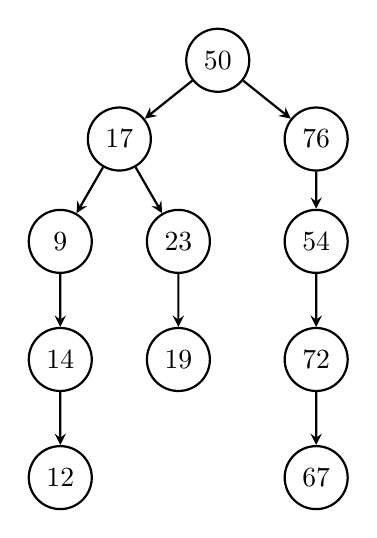
\begin{tikzpicture}[every node/.style={circle,draw, minimum size=8mm}, node distance=15mm, thick, ->, >=stealth]

\tikzstyle{level 1}=[level distance=10mm, sibling distance=2.5cm]
\tikzstyle{level 2}=[level distance=13mm, sibling distance=1.5cm]
\tikzstyle{level 3}=[level distance=15mm, sibling distance=1cm]
\tikzstyle{level 4}=[level distance=15mm, sibling distance=1cm]

\node {$50$}
   child{node {$17$}
             child{node {$9$}
				child{node {$14$}
					child{node {$12$}}				
				}             
             }
             child{node {$23$}
				child{node {$19$}}             
             }
        }
   child{node {$76$}
			child{node {$54$}
				child{node {$72$}
					child{node {$67$}}				
				}
			}
		};
\end{tikzpicture}
\caption{}
\label{unbalanced}
\end{subfigure}
\hspace{1em}
\begin{subfigure}[b]{0.4\linewidth}
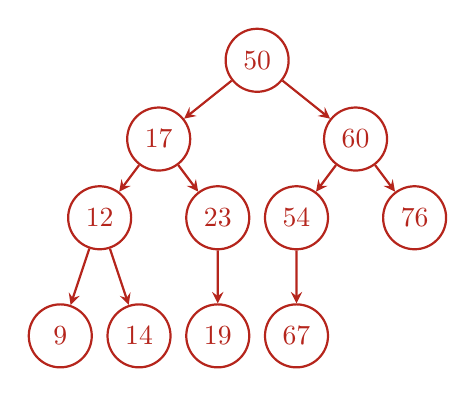
\begin{tikzpicture}[every node/.style={circle,draw, minimum size=8mm}, node distance=15mm, thick, ->, >=stealth, BrickRed]

\tikzstyle{level 1}=[level distance=10mm, sibling distance=2.5cm]
\tikzstyle{level 2}=[level distance=10mm, sibling distance=1.5cm]
\tikzstyle{level 3}=[level distance=15mm, sibling distance=1cm]
\tikzstyle{level 4}=[level distance=15mm, sibling distance=1cm]


\node {$50$}
   child{node {$17$}
             child{node {$12$}
				child{node {$9$}}
				child{node {$14$}}
			 }
             child{node {$23$}
				child{node {$19$}}             
             }
        }
   child{node {$60$}
			child{node {$54$}
				child{node {$67$}}
			}
			child{node {$76$}}
		};
\end{tikzpicture}
\caption{}
\label{balanced}
\end{subfigure}
\caption[Example of unbalanced (\ref{unbalanced}) and balanced (\ref{balanced}) tree.]{Example of unbalanced (\ref{unbalanced}) and balanced tree (\ref{balanced}). Credits: \href{https://en.wikipedia.org/wiki/Self-balancing_binary_search_tree}{Self-balancing binary search tree, Wikipedia}}
\label{trees_19}
\end{figure}

In Figure \ref{trees_19} is show an unbalanced tree (\ref{unbalanced}) in which the average path to reach the leaf is 3.27 nodes. If the same tree is balanced (\ref{balanced}) the average path to reach any leaf from the root decreased to 3.

\section{Red-Black Trees}
The \textbf{red-black trees} are particular kind of self balancing trees. An extra bit is used to store the color of the node, which can be only \textbf{red} or \textbf{black}. Using a color for each node assures that the tree remains balanced during insertion and deletion operations \cite{wikiblackred} (\href{https://en.wikipedia.org/wiki/Red%E2%80%93black_tree}{Red-black tree, Wikipedia}).

The rules that a red-black tree must respect are:
\begin{itemize}
\item[1] Nodes can be only of two types: \textbf{red} or \textbf{black}.
\item[2] There must exist the \textbf{null leaf nodes}. Every node which does not have two leaf must have the children \textbf{null}.
\item[3] If a node is \textbf{red} all its children must be \textbf{black}.
\item[4] Usually the root is \textbf{black}, but this is not mandatory.
\item[5] Every path from a the upper nodes to the lower ones must contain the same number of \textbf{black} nodes. This property is very important when inserting new nodes.
\end{itemize}

\begin{figure}[H]
\centering
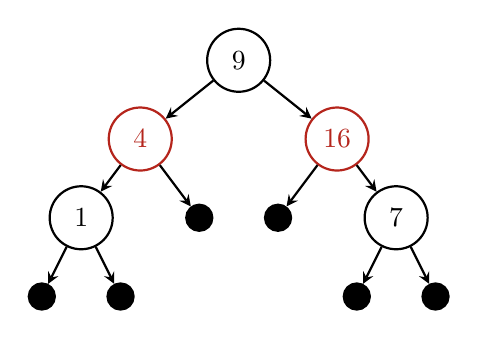
\begin{tikzpicture}[thick, every node/.style={circle,draw}, minimum size=8mm, ->, >=stealth]

\tikzstyle{level 1}=[level distance=10mm, sibling distance=2.5cm]
\tikzstyle{level 2}=[level distance=10mm, sibling distance=1.5cm]
\tikzstyle{level 3}=[level distance=10mm, sibling distance=1cm]
\tikzstyle{level 4}=[level distance=10mm, sibling distance=1cm]



\node {$9$}
   	child{node[shape=circle, text=BrickRed, fill=white, draw=BrickRed] {$4$}
		child{node {$1$}
			child{node[shape=circle, fill=black, minimum size=1mm] {}}
			child{node[shape=circle, fill=black, minimum size=1mm] {}}
		} 
		child{node[shape=circle, fill=black, minimum size=1mm] {}}	 			
   	}
    child{node[shape=circle, text=BrickRed, fill=white, draw=BrickRed] {$16$}
   	 	child{node[shape=circle, fill=black, minimum size=1mm] {}}
		child{node {$7$}
			child{node[shape=circle, fill=black, minimum size=1mm] {}}
			child{node[shape=circle, fill=black, minimum size=1mm] {}}		
		}
   	 };

\end{tikzpicture}
\caption[A red-black tree.]{A red-black tree.}
\label{trees_20}
\end{figure}

Usual only red nodes are added and the color of the other nodes are changed accordingly in order to respect the rule for the red-black tree.

\begin{figure}[H]
\centering
\begin{subfigure}[b]{0.4\linewidth}
\centering
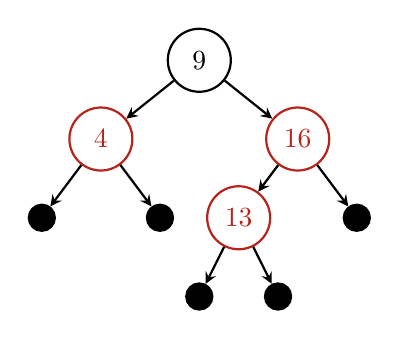
\begin{tikzpicture}[every node/.style={circle,draw, minimum size=8mm}, node distance=15mm, thick, ->, >=stealth]

\tikzstyle{level 1}=[level distance=10mm, sibling distance=2.5cm]
\tikzstyle{level 2}=[level distance=10mm, sibling distance=1.5cm]
\tikzstyle{level 3}=[level distance=10mm, sibling distance=1cm]
\tikzstyle{level 4}=[level distance=10mm, sibling distance=1cm]

\node {$9$}
   	child{node[shape=circle, text=BrickRed, fill=white, draw=BrickRed] {$4$}
		child{node[shape=circle, fill=black, minimum size=1mm] {}}
		child{node[shape=circle, fill=black, minimum size=1mm] {}}		
   	}
    child{node[shape=circle, text=BrickRed, fill=white, draw=BrickRed] {$16$}
    	child{node[shape=circle, text=BrickRed, fill=white, draw=BrickRed] {$13$}
			child{node[shape=circle, fill=black, minimum size=1mm] {}}
			child{node[shape=circle, fill=black, minimum size=1mm] {}}		
		}
   	 	child{node[shape=circle, fill=black, minimum size=1mm] {}}
   	 };
\end{tikzpicture}
\end{subfigure}
\hspace{1em}
\begin{subfigure}[b]{0.4\linewidth}
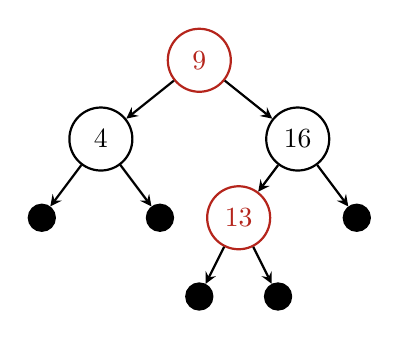
\begin{tikzpicture}[every node/.style={circle,draw, minimum size=8mm}, node distance=15mm, thick, ->, >=stealth]

\tikzstyle{level 1}=[level distance=10mm, sibling distance=2.5cm]
\tikzstyle{level 2}=[level distance=10mm, sibling distance=1.5cm]
\tikzstyle{level 3}=[level distance=10mm, sibling distance=1cm]
\tikzstyle{level 4}=[level distance=10mm, sibling distance=1cm]

\node[shape=circle, text=BrickRed, fill=white, draw=BrickRed] {$9$}
   	child{node {$4$}
		child{node[shape=circle, fill=black, minimum size=1mm] {}}
		child{node[shape=circle, fill=black, minimum size=1mm] {}}		
   	}
    child{node {$16$}
    	child{node[shape=circle, text=BrickRed, fill=white, draw=BrickRed] {$13$}
			child{node[shape=circle, fill=black, minimum size=1mm] {}}
			child{node[shape=circle, fill=black, minimum size=1mm] {}}		
		}
   	 	child{node[shape=circle, fill=black, minimum size=1mm] {}}
   	 };
\end{tikzpicture}
\end{subfigure}
\caption[Insertion of a new node and the following updating of the color nodes.]{Insertion of a new node and the following updating of the color nodes.}
\label{trees_21}
\end{figure}

In case the insertion or the removal does nor respect the rules of the red-black tree and BST some more complex operations must be done as in the following figure.

\begin{figure}[H]
\centering
\begin{subfigure}[b]{0.4\linewidth}
\centering
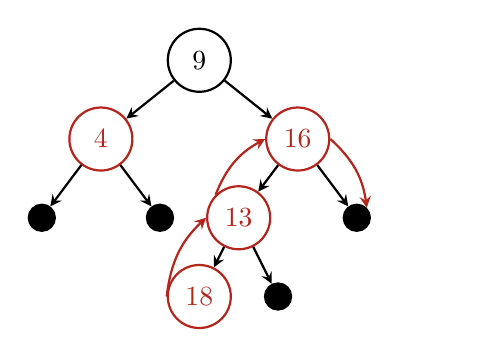
\begin{tikzpicture}[every node/.style={circle,draw, minimum size=8mm}, node distance=15mm, thick, ->, >=stealth]

\tikzstyle{level 1}=[level distance=10mm, sibling distance=2.5cm]
\tikzstyle{level 2}=[level distance=10mm, sibling distance=1.5cm]
\tikzstyle{level 3}=[level distance=10mm, sibling distance=1cm]
\tikzstyle{level 4}=[level distance=10mm, sibling distance=1cm]

\node {$9$}
   	child{node[shape=circle, text=BrickRed, fill=white, draw=BrickRed] {$4$}
		child{node[shape=circle, fill=black, minimum size=1mm] {}}
		child{node[shape=circle, fill=black, minimum size=1mm] {}}		
   	}
    child{node[shape=circle, text=BrickRed, fill=white, draw=BrickRed] (n16) {$16$}
    	child{node[shape=circle, text=BrickRed, fill=white, draw=BrickRed] (n13) {$13$}
			child{node[shape=circle, text=BrickRed, fill=white, draw=BrickRed] (n18) {$18$}}
			child{node[shape=circle, fill=black, minimum size=1mm] {}}		
		}
   	 	child{node[shape=circle, fill=black, minimum size=1mm] (ne) {}}
   	 };
\path[->, BrickRed] (n13.north west) edge [bend left=20] node[draw=none, xshift=24pt] {} (n16.west);
\path[->, BrickRed] (n18.west) edge [bend left=20] node[draw=none, xshift=24pt] {} (n13.west);
\path[->, BrickRed] (n16.east) edge [bend left=20] node[draw=none, xshift=24pt] {} (ne.north east);
\end{tikzpicture}
\end{subfigure}
\hspace{1em}
\begin{subfigure}[b]{0.4\linewidth}
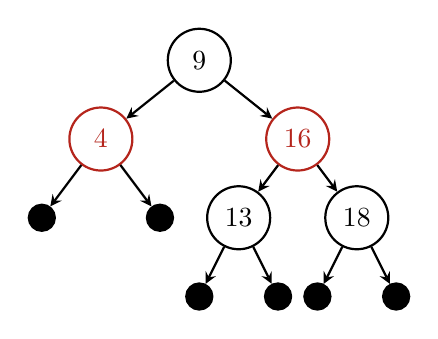
\begin{tikzpicture}[every node/.style={circle,draw, minimum size=8mm}, node distance=15mm, thick, ->, >=stealth]

\tikzstyle{level 1}=[level distance=10mm, sibling distance=2.5cm]
\tikzstyle{level 2}=[level distance=10mm, sibling distance=1.5cm]
\tikzstyle{level 3}=[level distance=10mm, sibling distance=1cm]
\tikzstyle{level 4}=[level distance=10mm, sibling distance=1cm]

\node {$9$}
   	child{node[shape=circle, text=BrickRed, fill=white, draw=BrickRed] {$4$}
		child{node[shape=circle, fill=black, minimum size=1mm] {}}
		child{node[shape=circle, fill=black, minimum size=1mm] {}}		
   	}
    child{node[shape=circle, text=BrickRed, fill=white, draw=BrickRed] (n16) {$16$}
    	child{node (n13) {$13$}
			child{node[shape=circle, fill=black, minimum size=1mm] {}}
			child{node[shape=circle, fill=black, minimum size=1mm] {}}    	
    	}
		child{node (n18) {$18$}
			child{node[shape=circle, fill=black, minimum size=1mm] {}}
			child{node[shape=circle, fill=black, minimum size=1mm] {}}		
		}
   	 };
\end{tikzpicture}
\end{subfigure}
\caption[An example of right rotation.]{An example of right rotation.}
\label{trees_22}
\end{figure}